\documentclass[12pt,a4paper]{article}
\usepackage[T1]{fontenc}
\usepackage[utf8]{inputenc}
\usepackage{graphicx} 
\usepackage{url}
\graphicspath{{images/}} 
\renewcommand{\figurename}{Şekil}
\renewcommand{\refname}{Kaynakça}
\usepackage{geometry}
\usepackage{hyperref}
\usepackage{subcaption}
\usepackage{amsmath}

\title{\bf\fontsize{12pt}{14pt}\selectfont KÜTAHYA SAĞLIK BİLİMLERİ ÜNİVERSİTESİ \\ MÜHENDİSLİK VE DOĞA BİLİMLERİ FAKÜLTESİ}
\date{}
\begin{document}
	
	\maketitle
	\begin{center}
			
\includegraphics[width=0.25\linewidth]{ksbu.png}
	\end{center}
	\begin{center}
	\end{center}
	\begin{center}
	\title{\bf\fontsize{12pt}{14pt}\selectfont YAPAY ZEKA DERSİ FİNAL RAPORU }
	\end{center}
		\begin{center}
		\title{\bf\fontsize{12pt}{14pt}\selectfont Sistem LOG dosyalarını inceleyerek, sistemde aktif ya da öncesinde
var olmuş yetkisiz girişlerin tespit edilmesi}
        \end{center}
	\begin{center}
	\end{center}
	\begin{center}
		
	
	\author{\bf\fontsize{12pt}{14pt}Barış AZAR \hspace{1.5cm}2118121004}
	
	\begin{center}
	\end{center}
  \bf\fontsize{12pt}{14pt}\selectfont {Anahtar kelimeler: LOG Analizi, LSTM, Yapay Zeka, Access.log\newline}
    \begin{abstract}
Bu çalışmada, yetkisiz girişleri tespit etmek amacıyla yapay zeka teknolojilerinden yararlanılarak bir log analiz sistemi geliştirilmiştir.
Çalışmanın temel amacı, hem içeriden hem de dışarıdan yapılan yetkisiz erişim girişimlerini, sunucu erişim logları üzerinden analiz ederek belirlemektir.
Farklı senaryolar ve yapay zeka modelleriyle, bu verilerin yapay zeka modelleriyle işlenmesi sonucu yetkisiz erişim girişimlerinin tespit edilip edilemeyeceği araştırılmıştır.
Sonuç olarak, bu çalışma, log dosyalarının yapay zeka yardımıyla analiz edilerek sistem güvenliğinin nasıl artırılabileceğine dair önemli bilgiler sunmaktadır.    \end{abstract}

	\end{center}

  \newpage
	\section{Giriş}
Güvenlik, günümüzde dijital sistemler için kritik bir öneme sahiptir. Yapılan araştırmaya göre, 2023 yılında küresel çapta 2.365 siber saldırı yaşanmış ve bu saldırılar sonucunda 343.338.964 kişi etkilenmiştir. Saldırılardan kaynaklanan veri ihlallerinin ortalama maliyeti 4.45 milyon USD olmuştur. Saldırıların etkisi ve maliyeti düşünülünce siber güvenlik alanında yatırımlar ve veri sızmasını engellemek için çalışmaların olması hayatidir.\cite{Cyber_attack}\newline\newline Çalışmanın amacı yüksek güvenlikli sunucu ve kritik sistemleri ve o sunuculara içeriden erişebilen çalışan yönetici vb. kişilerin şahsi ve kurumsal bilgisayarlarında keşif yapmayı amaçlamaktadır. Çalışmanın önemi, araştırmacının Yapay Zeka, log analizi konusunda tecrübe sağlaması ve bu tecrübelerin temel aldığı farklı çalışmalar yapmasına katkı sağlamaktır. Literatür açısından, yapay zeka ile log analizi konusunda farklı yapay zeka modellerini karşılaştırmak önemli bir katkıdır. Çalışmada, sistem güvenliğini artırmak amacıyla yapay zeka kullanarak sistemde aktif olarak işlem yapan ya da geçmişte işlem yapmış izinsiz girişleri tespit etmek amacıyla geliştirilmektedir. Sistem erişim (access) log dosyalarını analiz edilerek çıktı üretilmesi üzerine çalışılmaktadır.

\section{Veri Seti}
Veri seti, "Kirli" ve "Temiz" olarak 2 adet kategori mevcuttur. Kirli veri seti çalışma için özel olarak elde edilmiştir. Kirli veri setini hazırlamak için yerel ağ üzerinden Apache sunucu sistemi üzerine saldırı gerçekleştirilmiştir \cite{Dirbuster},\cite{gobuster}. Saldırı türü wordlist'dir. Wordlist olarak \cite{big.txt} kullanılmıştır. Saldırı sonucunda oluşan access.log dosyası kirli verileri oluşturmaktadır. Karşıt olarak temiz verisi için \cite{kaggle} verileri kullanılmıştır.

Toplamda 20.000 adet veri mevcuttur. Bu veriler \%70 eğitim (14.000 veri), \%20 test (4.000 veri) ve \%10 doğrulama (2.000 veri) olacak şekilde ayrılmıştır. Kirli ve temiz veri setleri dengeli olarak dağıtılmış ve analiz edilmiştir. Eğitim seti, modeli saldırıları tanımlamak üzere eğitirken, test seti modelin performansını değerlendirir. Doğrulama seti ise modelin hiperparametrelerini optimize etmek için kullanılmıştır. Bu yaklaşım, modelin gerçek dünya saldırılarını tanıyabilmesi ve yanıltıcı pozitifleri minimize etmesi için tasarlanmıştır. Eğitim seti üzerinde modelin öğrenme süreci, saldırı tespit performansını maksimize edecek şekilde yürütülmüştür.

\section{Yöntem}
\subsection{Yapay Zeka Modeli}

Bu çalışma kapsamında, bir LSTM (Long Short-Term Memory) tabanlı model kullanarak log verilerini analiz eden ve zararlı etkinlikleri tespit eden bir derin öğrenme modeli oluşturulmuştur. Bu model, metin verilerini işleyip sınıflandırarak hangi logların saldırıya uğradığını (infected) ve hangilerinin temiz olduğunu (not infected) belirlemektedir. Aşağıda, modelin her bir bileşeni ve adımı detaylı olarak açıklanmaktadır.

\subsubsection{Veri Hazırlığı ve Yükleme}

Çalışmanın ilk adımı, gerekli veri setlerini ve anahtar kelimeleri yüklemektir. Log verileri, bir Excel dosyasından alınmış ve her bir log girdisi metin formatında bir listeye dönüştürülmüştür. Bu log verileri, saldırı girişimlerini ve normal etkinlikleri içermektedir. Yüklenen veriler, gereksiz bilgilerin çıkarılması amacıyla temizlenmiştir. Bu temizlik işlemi, her bir log girdisinden ilk virgülden sonraki kısmı alarak gerçekleştirilmiştir. Böylece, analiz edilecek log metinlerinin sadece önemli kısımları elde edilmiştir.

Anahtar kelimeler, bir metin dosyasından yüklenmiştir. Bu anahtar kelimeler, saldırı tespitinde kullanılacak kritik kelimeleri içerir ve her satır bir anahtar kelime olacak şekilde listeye dönüştürülmüştür. Bu sayede, log verilerinde bu anahtar kelimelerin varlığına göre etiketleme yapılması sağlanmıştır.

\subsubsection{Veri Etiketleme}

Veri etiketleme işlemi, log verilerinde anahtar kelimelerin bulunup bulunmadığını kontrol ederek gerçekleştirilmiştir. Eğer bir log girdisinde herhangi bir anahtar kelime bulunuyorsa, bu log girdisi "infected" (saldırıya uğramış) olarak etiketlenmiştir. Aksi halde, log girdisi "not infected" (saldırıya uğramamış) olarak işaretlenmiştir. Bu etiketleme işlemi, saldırı tespiti için gerekli olan denetimli öğrenme modelinin eğitiminde kullanılacak veri setini oluşturmuştur.

\subsubsection{Metin Verisinin İşlenmesi}

Log verilerini makine öğrenmesi modeli için uygun hale getirmek amacıyla, metin verisi tokenize edilmiştir. Tokenizasyon işlemi, metinlerin kelime dizilerine dönüştürülmesini sağlar. Daha sonra bu diziler, modelin girdi olarak kullanabileceği sabit uzunlukta vektörler haline getirilmiştir. Bu işlem, tüm log girdilerinin aynı uzunlukta olmasını sağlayarak modelin düzgün bir şekilde eğitilmesini sağlamaktadır.

\subsubsection{Modelin Tanımlanması}

Modelin tanımlanması aşamasında, LSTM (Long Short-Term Memory) tabanlı bir sinir ağı modeli oluşturulmuştur. Bu model, metin verilerini işleyerek hangi logların saldırıya uğradığını tahmin etmeyi amaçlar. Modelin girdi katmanı, metin verilerini almak üzere tanımlanmıştır. Girdi verileri, embedding katmanı aracılığıyla sayısal bir temsile dönüştürülmüştür. Bu embedding katmanı, kelimelerin vektör temsilini öğrenerek metin verisinin anlamlı bir şekilde işlenmesini sağlar. Embedding katmanının çıktısı, LSTM katmanına aktarılmıştır. LSTM katmanı, zaman serisi verisi olan metinlerdeki ardışık ilişkileri öğrenir. Son olarak, dense katmanı kullanılarak modelin çıktısı üretilmiş ve bu çıktı, saldırı tespitinin yapılmasını sağlamaktadır.

\subsubsection{Modelin Eğitilmesi}

Modelin eğitimi için derleme işlemi yapılmış ve modelin optimize edilmesi amacıyla gerekli parametreler belirlenmiştir. Model, 'adam' optimizasyon algoritması ve 'binary\_crossentropy' kayıp fonksiyonu ile derlenmiştir. Modelin performansı, eğitim ve doğrulama doğruluğu ile değerlendirilmiştir. Eğitim süreci boyunca model, verinin \%70'i ile eğitilirken, \%20'si ile test edilmiş ve \%10'u doğrulama için kullanılmıştır. Eğitim sürecinde model, her epoch sonunda eğitim ve doğrulama kayıplarını ve doğruluklarını hesaplamıştır.

\section{Bulgu ve Tartışma}
\subsection{Metrikler}
\subsubsection{Doğru Pozitif (TP)}
\quad Gerçekte pozitif olan ve modelin de pozitif olarak tahmin ettiği örnekler.

\subsubsection{Doğru Negatif (TN)}
\quad Gerçekte negatif olan ve modelin de negatif olarak tahmin ettiği örnekler.

\subsubsection{Yanlış Pozitif (FP)}
\quad Gerçekte negatif olan ancak modelin pozitif olarak tahmin ettiği örnekler.

\subsubsection{Yanlış Negatif (FN)}
\quad Gerçekte pozitif olan ancak modelin negatif olarak tahmin ettiği örnekler.

\begin{figure}[!htbp]
    \centering
    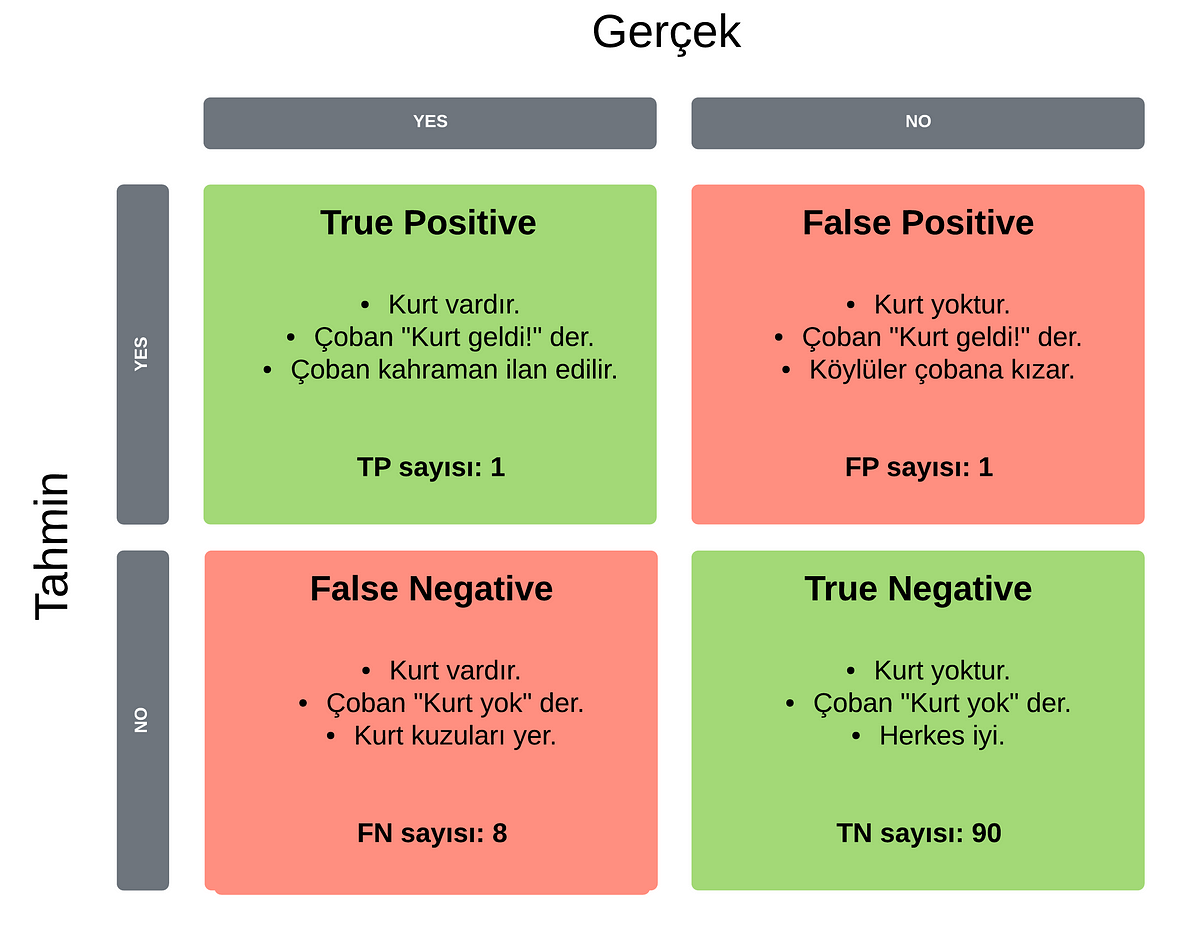
\includegraphics[width=1\linewidth]{metrik_aciklama.png}
    \caption{Metrik açıklayıcı görsel\cite{Metrik}.}
    \label{fig:enter-label}
\end{figure}\newpage

\subsubsection{Doğruluk (Accuracy}
\quad Modelin doğru tahminlerinin tüm tahminlere oranı.
\begin{align}
Dogruluk &= \frac{TP+TN}{TP+TN+FP+FN}
\end{align}

\subsubsection{Hassasiyet (Precision)}
\quad Pozitif olarak tahmin edilen örneklerin gerçekten pozitif olma oranı.
\begin{align}
Hassasiyet (Precision) &= \frac{TP}{TP+FP}
\end{align}

\subsubsection{Duyarlılık (Recall)}
\quad Gerçekte pozitif olan örneklerin model tarafından pozitif olarak tahmin edilme oranı.
\begin{align}
Duyarlilik (Recall) &= \frac{TP}{TP+FN}
\end{align}


\subsubsection{F1 Skoru (F1 Score)}
\quad Hassasiyet ve duyarlılığın harmonik ortalaması, modelin genel performansını değerlendirmek için kullanılır.
\begin{align}
F1 Skor &= 2 \cdot \frac{Hassasiyet \cdot Duyarlilik}{Hassasiyet + Duyarlilik}
\end{align}

\section{Sonuç}
Bu çalışmada, Apache sunucu sistemine yönelik saldırıların tespiti amacıyla bir LSTM tabanlı yapay zeka modeli geliştirilmiştir. Model, log verilerini analiz ederek zararlı etkinlikleri belirlemiş ve bu sayede sistem güvenliğini artırmak için önemli bir araç sunmuştur. Eğitim sürecinde modelin performansı çeşitli metriklerle değerlendirilmiştir. 

\begin{figure}[!htbp]
    \centering
    \includegraphics[width=1\linewidth]{GRAPHİCS.png}
    \caption{Eğitim - Doğrulama kayıp ve Eğitim - Doğrulama kesinlik grafiği}
    \label{fig:enter-label}
\end{figure}

Elde edilen sonuçlar, modelin yüksek doğruluk, hassasiyet, duyarlılık ve F1 skoru ile başarılı bir performans sergilediğini göstermiştir. Model, test verileri üzerinde \%97 doğruluk, \%92 hassasiyet, \%94 duyarlılık ve \%94 F1 skoru ile doğru ve güvenilir tahminler yapabilmiştir. Bu bulgular, log dosyalarının yapay zeka yardımıyla analiz edilerek izinsiz girişlerin tespit edilmesinin mümkün olduğunu ortaya koymaktadır. Gelecekteki çalışmalar, daha büyük ve çeşitli veri setleri ile modelin genelleme yeteneğinin artırılmasını hedefleyebilir.

\begin{table}[!htbp]
    \centering
    \caption{Eğitimde elde edilen sonuçlar}
    \begin{tabular}{|c|c|}
    \hline
    \textbf{Ölçüm metrikleri} & \textbf{Değerler} \\
    \hline
    True Positives & 22 \\
    \hline
    True Negatives & 75 \\
    \hline
    False Positives & 2 \\
    \hline
    False Negatives & 1 \\
    \hline
    Accuracy & 0.97 \\
    \hline
    Precision & 0.92 \\
    \hline
    Recall & 0.94 \\
    \hline
    F1 Score & 0.94 \\
    \hline
    \end{tabular}
\end{table}

\bibliographystyle{ieeetr}
\bibliography{./sample.bib}
\end{document}
